%File: formatting-instructions-latex-2024.tex
%release 2024.0
\documentclass[letterpaper]{article} % DO NOT CHANGE THIS
\usepackage[submission]{aaai24}  % DO NOT CHANGE THIS
\usepackage{times}  % DO NOT CHANGE THIS
\usepackage{helvet}  % DO NOT CHANGE THIS
\usepackage{courier}  % DO NOT CHANGE THIS
\usepackage[hyphens]{url}  % DO NOT CHANGE THIS
\usepackage{graphicx} % DO NOT CHANGE THIS
\urlstyle{rm} % DO NOT CHANGE THIS
\def\UrlFont{\rm}  % DO NOT CHANGE THIS
\usepackage{natbib}  % DO NOT CHANGE THIS AND DO NOT ADD ANY OPTIONS TO IT
\usepackage{caption} % DO NOT CHANGE THIS AND DO NOT ADD ANY OPTIONS TO IT
\frenchspacing  % DO NOT CHANGE THIS
\setlength{\pdfpagewidth}{8.5in}  % DO NOT CHANGE THIS
\setlength{\pdfpageheight}{11in}  % DO NOT CHANGE THIS
%
% These are recommended to typeset algorithms but not required. See the subsubsection on algorithms. Remove them if you don't have algorithms in your paper.
\usepackage{algorithm}
\usepackage{algorithmic}

%
% These are are recommended to typeset listings but not required. See the subsubsection on listing. Remove this block if you don't have listings in your paper.
\usepackage{newfloat}
\usepackage{listings}
\DeclareCaptionStyle{ruled}{labelfont=normalfont,labelsep=colon,strut=off} % DO NOT CHANGE THIS
\lstset{%
	basicstyle={\footnotesize\ttfamily},% footnotesize acceptable for monospace
	numbers=left,numberstyle=\footnotesize,xleftmargin=2em,% show line numbers, remove this entire line if you don't want the numbers.
	aboveskip=0pt,belowskip=0pt,%
	showstringspaces=false,tabsize=2,breaklines=true}
\floatstyle{ruled}
\newfloat{listing}{tb}{lst}{}
\floatname{listing}{Listing}
%
% Keep the \pdfinfo as shown here. There's no need
% for you to add the /Title and /Author tags.
\pdfinfo{
/TemplateVersion (2024.1)
}

% DISALLOWED PACKAGES
% \usepackage{authblk} -- This package is specifically forbidden
% \usepackage{balance} -- This package is specifically forbidden
% \usepackage{color (if used in text)
% \usepackage{CJK} -- This package is specifically forbidden
% \usepackage{float} -- This package is specifically forbidden
% \usepackage{flushend} -- This package is specifically forbidden
% \usepackage{fontenc} -- This package is specifically forbidden
% \usepackage{fullpage} -- This package is specifically forbidden
% \usepackage{geometry} -- This package is specifically forbidden
% \usepackage{grffile} -- This package is specifically forbidden
% \usepackage{hyperref} -- This package is specifically forbidden
% \usepackage{navigator} -- This package is specifically forbidden
% (or any other package that embeds links such as navigator or hyperref)
% \indentfirst} -- This package is specifically forbidden
% \layout} -- This package is specifically forbidden
% \multicol} -- This package is specifically forbidden
% \nameref} -- This package is specifically forbidden
% \usepackage{savetrees} -- This package is specifically forbidden
% \usepackage{setspace} -- This package is specifically forbidden
% \usepackage{stfloats} -- This package is specifically forbidden
% \usepackage{tabu} -- This package is specifically forbidden
% \usepackage{titlesec} -- This package is specifically forbidden
% \usepackage{tocbibind} -- This package is specifically forbidden
% \usepackage{ulem} -- This package is specifically forbidden
% \usepackage{wrapfig} -- This package is specifically forbidden
% DISALLOWED COMMANDS
% \nocopyright -- Your paper will not be published if you use this command
% \addtolength -- This command may not be used
% \balance -- This command may not be used
% \baselinestretch -- Your paper will not be published if you use this command
% \clearpage -- No page breaks of any kind may be used for the final version of your paper
% \columnsep -- This command may not be used
% \newpage -- No page breaks of any kind may be used for the final version of your paper
% \pagebreak -- No page breaks of any kind may be used for the final version of your paperr
% \pagestyle -- This command may not be used
% \tiny -- This is not an acceptable font size.
% \vspace{- -- No negative value may be used in proximity of a caption, figure, table, section, subsection, subsubsection, or reference
% \vskip{- -- No negative value may be used to alter spacing above or below a caption, figure, table, section, subsection, subsubsection, or reference

\setcounter{secnumdepth}{0} %May be changed to 1 or 2 if section numbers are desired.

% The file aaai24.sty is the style file for AAAI Press
% proceedings, working notes, and technical reports.
%

% Title

% Your title must be in mixed case, not sentence case.
% That means all verbs (including short verbs like be, is, using,and go),
% nouns, adverbs, adjectives should be capitalized, including both words in hyphenated terms, while
% articles, conjunctions, and prepositions are lower case unless they
% directly follow a colon or long dash
\title{MEDIAIT: A Modular Environment for Driving Insights in Automated Interactive Theorem-Proving}
\author{
    %Authors
    % All authors must be in the same font size and format.
    Written by AAAI Press Staff\textsuperscript{\rm 1}\thanks{With help from the AAAI Publications Committee.}\\
    AAAI Style Contributions by Pater Patel Schneider,
    Sunil Issar,\\
    J. Scott Penberthy,
    George Ferguson,
    Hans Guesgen,
    Francisco Cruz\equalcontrib,
    Marc Pujol-Gonzalez\equalcontrib
}
\affiliations{
    %Afiliations
    \textsuperscript{\rm 1}Association for the Advancement of Artificial Intelligence\\
    % If you have multiple authors and multiple affiliations
    % use superscripts in text and roman font to identify them.
    % For example,

    % Sunil Issar\textsuperscript{\rm 2}, 
    % J. Scott Penberthy\textsuperscript{\rm 3}, 
    % George Ferguson\textsuperscript{\rm 4},
    % Hans Guesgen\textsuperscript{\rm 5}
    % Note that the comma should be placed after the superscript

    1900 Embarcadero Road, Suite 101\\
    Palo Alto, California 94303-3310 USA\\
    % email address must be in roman text type, not monospace or sans serif
    proceedings-questions@aaai.org
%
% See more examples next
}

%Example, Single Author, ->> remove \iffalse,\fi and place them surrounding AAAI title to use it
\iffalse
\title{My Publication Title --- Single Author}
\author {
    Author Name
}
\affiliations{
    Affiliation\\
    Affiliation Line 2\\
    name@example.com
}
\fi

\iffalse
%Example, Multiple Authors, ->> remove \iffalse,\fi and place them surrounding AAAI title to use it
\title{My Publication Title --- Multiple Authors}
\author {
    % Authors
    First Author Name\textsuperscript{\rm 1,\rm 2},
    Second Author Name\textsuperscript{\rm 2},
    Third Author Name\textsuperscript{\rm 1}
}
\affiliations {
    % Affiliations
    \textsuperscript{\rm 1}Affiliation 1\\
    \textsuperscript{\rm 2}Affiliation 2\\
    firstAuthor@affiliation1.com, secondAuthor@affilation2.com, thirdAuthor@affiliation1.com
}
\fi


% REMOVE THIS: bibentry
% This is only needed to show inline citations in the guidelines document. You should not need it and can safely delete it.
\usepackage{bibentry}
% END REMOVE bibentry

\begin{document}

\maketitle

\begin{abstract}
    Recent interest in Artificial Intelligence for Theorem Proving (AITP) has given rise to a plethora of benchmarks and
    methodologies,
    particularly in the area of Interactive Theorem Proving (ITP).
    Research in the area is fragmented, with a diverse set of approaches being spread across several ITP systems.
    This presents a significant challenge to the comparison of methods, which are often complex and difficult to replicate.
    To address this, we present MEDIAIT: A Modular Environment for Driving Insights in Automaing Interactive Theorem-proving.
    By separating the learning approach from the data and ITP environment, MEDIAIT allows for the fair and efficient
    comparison of approaches between systems.
    MEDIAIT is designed to seamlessly incorporate new systems and benchmarks, currently integrating the HOList, HOLStep,
    MIZAR40, LeanStep, LeanGym and TacticZero benchmarks.
    We demonstrate the utility of MEDIAIT through a study of embedding architectures in the context of the above systems.
     % (Through comparing the performance of approaches across a variety of ITP settings, we provide strong evidence that..)
    These experiments lay the foundations for future work in evaluation of performance of formula embedding,
    while simultaneously demonstrating the capability of the framework.
     % (We show that the embedding approach of HOList applied to HOL4's TacticZero provides a significant improvement in)
     % (performance.)
    We complement these with a qualitative analysis of embeddings within and between systems, illustrating that improved
    performance was associated with more semantically aware embeddings.
    By streamlining the implementation and comparison of Machine Learning algorithms in the ITP context,
    we anticipate MEDIAIT will be a springboard for future
    research.

\end{abstract}

\section{Introduction}

Interactive Theorem Proving (ITP) is a key paradigm of formal verification.
With a human providing high level proof guidance, ITP systems have been used to develop verified compilers (cite), formalise mathematical conjectures (cite) and develop provably correct microkernels (cite).
Successful proof guidance requires proficiency in both the formal system and the application domain.
This has limited the scale and widespread adoption of formal methods, with e.g...
The nascent field of Artificial Intelligence for Theorem Proving (AITP) has the potential to address this,
with several strong results in automating human ITP guidance.
AITP research encompasses several mathematical reasoning tasks, such as math word problems (cite) and autoformalisation (cite).
The focus of this paper is specifially AI for Interactive Theorem Proving, which we refer to as AI-ITP.

Current datasets and environments for AI-ITP are divided across several distinct ITP systems.
Although this provides a variety of tasks for benchmarking,
it poses a challenge to the fair and efficient comparison of the automation approaches.
This is further complicated by the broad range of methods which have been applied in the area,
which are generally tested only in the context of a single ITP system (cite).
(examples, HOList over the HOL Light prover, LeanStep/LeanGym over Lean,
TacticZero and TacticToe,.. with HOL4).

% (Current benchmarks have made significant progress in the generation of quality ITP proof data,)
% (still small in the context of large models and compared to NLP. )
% (Through curating these data sources into a centralised platform, we have created a large dataset  of xxx examples and xxx GB of proof data.)

A central component of AI-ITP systems is their embedding model.
Vector embeddings of the ITP logical expressions are required for the application of learning algorithms.
These are used for tasks such as premise selection, goal selection which are essential for proof guidance.

Expressions are either treated as a natural language sequence, or as a directed graph derived from their abstract syntax tree
representation. It has been argued that a graph representation is more appropriate, with a large body of work in AI-ITP
using Graph Neural Network (GNN) as the embedding model to achieve strong results in several tasks.

However, Transformer models applied to the sequence representation have also demonstrated strong performance by
leveraging large models pre-trained on NLP datasets.

Both architectures have fundamental limitations, as GNNs suffer from poor integration of global information, and vanlla
Transformers ignore the structural information of the expression.
Recent work has shown that combining both architectures leads to improved performance on several graph learning tasks.
In the context of theorem proving however, there has been no thorough comparison between approaches.

We address these two issues by ... our contributions can be summarised as ...

\subsection{Related Work}
Unified toolkit proposed for MWP, MWPToolkit.

- However, AI for ITP has several additional considerations:
- Fundamentally different learning approaches. Range from E2E RL, direct supervised learning, pretrained LLMs ..
- Makes it difficult to be fully modular as there are some unavoidable dependencies between e.g. environment and
model (e.g. HOL4 environment for TacticZero)
- Interaction with an environment
- Several axes of variation in algorithm design. Learning paradigm, proof search, embedding arch., action selection
arch.

Note we restrict ourselves to the problem of automating the human interaction with ITP, through the setup in Figure x.
Other approaches such as ML for Hammers, also promising

AIITP benchmarks mentioned, limited in single system.
Other unified frameworks, e.g. NLP, CV, GNN (graph benchmarks), which have provided strong value to their respective areas

\section{Background}
\subsection{ITP}
% - Lean, metamath (mizar), HOL4, HOL-Light
\subsection{Approaches}
\begin{figure}[h]
    \centering
    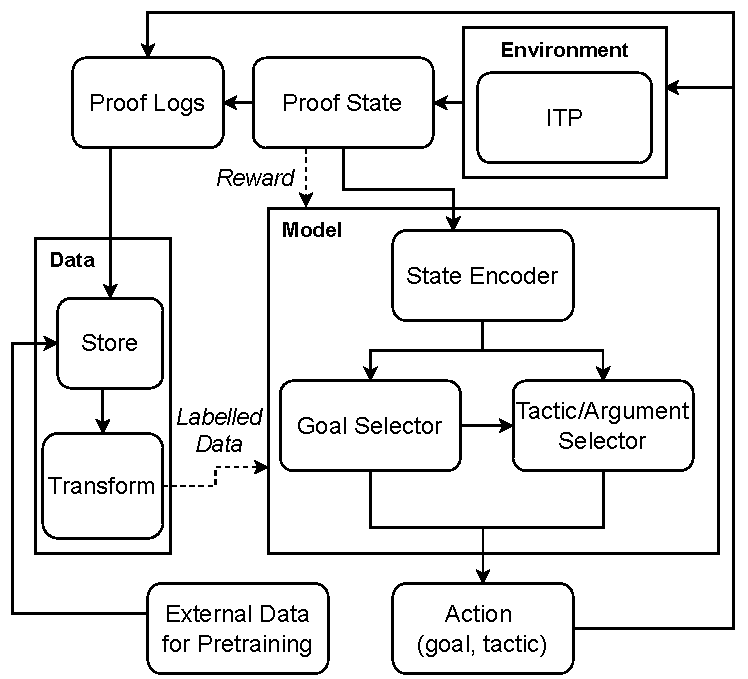
\includegraphics[width=\linewidth]{AI-ITP}
    \caption{Caption for the figure.}
    \label{fig:ai-itp}
\end{figure}
\subsubsection{Learning Approach}
RL (Policy Gradient) end to end,
Supervised Training over labelled proof logs (tactic, premise, goal),
Pre-training over proof data (PACT)
Pre-training over NLP corpus
\subsubsection{Proof Search}
BFS, Fringe, HyperTree MCTS
\subsubsection{State Embedding}
Transformer, GNN, SAT, Directed SAT, Autoencoder
\subsubsection{Tactic Selection}
Fixed set of tactics/arguments (TacticZero, HOList), generative model (GPT-f, Curriculum learning, lean)

%
\subsection{Datasets and Benchmarks}
%- LeanStep, mizar40, mizar60?, HOLStep,
%- Environments
%- HOList, LeanGym, CoqGym, HOL4

Figure (Table):
Benchmark vs Details (size, system, interactive)
Highlight in bold what is currently included
Include HOL4 premise selection
HOList, LeanStep, HOLStep, MIZAR40, LeanGym, TacticZero, (CoqGym, IsarStep etc from survey)

As outlined in Figure x, benchmarks consider each system in isolation, and generally focus on a small set of
learning and proof search approaches.
Given the many differences between ITPs, this is unsurprising, as there is significant effort required to set
up these systems for automated proving.

%HOList provides a large scale dataset and interactive environment for HOL Light, with a Breadth First Search proof large
%scale dataset and interactive environment for HOL Light, with a Breadth First Search proof
%
%and LeanStep/LeanGym are the two largest and
%

\subsection{Embedding Architecture}

Figure (Table):
Interactive Approaches vs Details
Proof search
BFS, MCTS, Fringe
Embedding architecture
GNN, Transformer, Autoencoder
Tactic/Argument selection
Generative (lean, hypertree), Fixed set (HOL4, HOList)
Learning approach
RL (TacticZero), Supervised proof logs (HOList, Lean, Hypertree?)

\section{MEDIATE}
Diagram and explanation of system architecture,

Open Source additions:
LeanGym/LeanStep output s-expressions
HOList using non-google tools, and independent of TF1 and ML framework

Curated, large dataset of varied ITPs

Modular framework

\section{Embedding Experiments}
\subsection{Supervised}
MIZAR, HOLStep, HOL4 pretrain, HOList Pretrain, Lean?
\subsection{End to End}
TacticZero, HOList
\subsection{Qualitative Analysis}
\section{Discussion}
\section{Conclusion}

%
%\section{Additional Resources}
%\LaTeX{} is a difficult program to master. If you've used that software, and this document didn't help or some items were not explained clearly, we recommend you read Michael Shell's excellent document (testflow doc.txt V1.0a 2002/08/13) about obtaining correct PS/PDF output on \LaTeX{} systems. (It was written for another purpose, but it has general application as well). It is available at www.ctan.org in the tex-archive.
%
%\appendix
%\section{Reference Examples}
%\label{sec:reference_examples}
%
%\nobibliography*
%Formatted bibliographies should look like the following examples. You should use BibTeX to generate the references. Missing fields are unacceptable when compiling references, and usually indicate that you are using the wrong type of entry (BibTeX class).
%
%\paragraph{Book with multiple authors~\nocite{em:86}} Use the \texttt{@book} class.\\[.2em]
%\bibentry{em:86}.
%
%\paragraph{Journal and magazine articles~\nocite{r:80, hcr:83}} Use the \texttt{@article} class.\\[.2em]
%\bibentry{r:80}.\\[.2em]
%\bibentry{hcr:83}.
%
%\paragraph{Proceedings paper published by a society, press or publisher~\nocite{c:83, c:84}} Use the \texttt{@inproceedings} class. You may abbreviate the \emph{booktitle} field, but make sure that the conference edition is clear.\\[.2em]
%\bibentry{c:84}.\\[.2em]
%\bibentry{c:83}.
%
%\paragraph{University technical report~\nocite{r:86}} Use the \texttt{@techreport} class.\\[.2em]
%\bibentry{r:86}.
%
%\paragraph{Dissertation or thesis~\nocite{c:79}} Use the \texttt{@phdthesis} class.\\[.2em]
%\bibentry{c:79}.
%
%\paragraph{Forthcoming publication~\nocite{c:21}} Use the \texttt{@misc} class with a \texttt{note="Forthcoming"} annotation.
%\begin{quote}
%\begin{footnotesize}
%\begin{verbatim}
%@misc(key,
%  [...]
%  note="Forthcoming",
%)
%\end{verbatim}
%\end{footnotesize}
%\end{quote}
%\bibentry{c:21}.
%
%\paragraph{ArXiv paper~\nocite{c:22}} Fetch the BibTeX entry from the "Export Bibtex Citation" link in the arXiv website. Notice it uses the \texttt{@misc} class instead of the \texttt{@article} one, and that it includes the \texttt{eprint} and \texttt{archivePrefix} keys.
%\begin{quote}
%\begin{footnotesize}
%\begin{verbatim}
%@misc(key,
%  [...]
%  eprint="xxxx.yyyy",
%  archivePrefix="arXiv",
%)
%\end{verbatim}
%\end{footnotesize}
%\end{quote}
%\bibentry{c:22}.
%
%\paragraph{Website or online resource~\nocite{c:23}} Use the \texttt{@misc} class. Add the url in the \texttt{howpublished} field and the date of access in the \texttt{note} field:
%\begin{quote}
%\begin{footnotesize}
%\begin{verbatim}
%@misc(key,
%  [...]
%  howpublished="\url{http://...}",
%  note="Accessed: YYYY-mm-dd",
%)
%\end{verbatim}
%\end{footnotesize}
%\end{quote}
%\bibentry{c:23}.
%
%For the most up to date version of the AAAI reference style, please consult the \textit{AI Magazine} Author Guidelines at \url{https://aaai.org/ojs/index.php/aimagazine/about/submissions#authorGuidelines}
%
%\section{Acknowledgments}
%AAAI is especially grateful to Peter Patel Schneider for his work in implementing the original aaai.sty file, liberally using the ideas of other style hackers, including Barbara Beeton. We also acknowledge with thanks the work of George Ferguson for his guide to using the style and BibTeX files --- which has been incorporated into this document --- and Hans Guesgen, who provided several timely modifications, as well as the many others who have, from time to time, sent in suggestions on improvements to the AAAI style. We are especially grateful to Francisco Cruz, Marc Pujol-Gonzalez, and Mico Loretan for the improvements to the Bib\TeX{} and \LaTeX{} files made in 2020.
%
%The preparation of the \LaTeX{} and Bib\TeX{} files that implement these instructions was supported by Schlumberger Palo Alto Research, AT\&T Bell Laboratories, Morgan Kaufmann Publishers, The Live Oak Press, LLC, and AAAI Press. Bibliography style changes were added by Sunil Issar. \verb+\+pubnote was added by J. Scott Penberthy. George Ferguson added support for printing the AAAI copyright slug. Additional changes to aaai24.sty and aaai24.bst have been made by Francisco Cruz, Marc Pujol-Gonzalez, and Mico Loretan.
%
%\bigskip
%\noindent Thank you for reading these instructions carefully. We look forward to receiving your electronic files!
%

\bibliography{aaai24}

\end{document}
